%
% sezione sulla convoluzione
%

\section{L'operazione di convoluzione\label{sec:convolution}}

L'operazione di convoluzione \`e la somma di una sorta di moltiplicazione
``scorrevole'' di un segnale con una data risposta all'impulso.
In pratica, questa operazione permette di analizzare il contributo della
moltiplicazione di ciascun campione del segnale
a un dato tempo $t$
con \emph{tutti} i campioni della risposta all'impulso.

Per esempio: il contributo della moltiplicazione della
risposta all'impulso $h_t$ con il campione $x_0$ al tempo $t$ sar\`a:

\begin{equation}
  x_0 h_t
\end{equation}

mentre quella del campione $t_1$ al tempo $t$ sar\`a:

\begin{equation}
  x_1 h_{t-1}
\end{equation}

ecc.

Quindi, tipicamente il contributo della moltiplicazione della risposta
all'impulso con il segnale $x_k$ \`e $x_k h_{t-k}$.

Dato che gestiamo sistemi lineari, possiamo sommare insieme tutti questi
contributi per avere il risultato finale:

\begin{equation}\label{eqn:generic convolution}
  y_t = \sum_{k = -\inf}^{\inf}{x_k h_{t-k}}
\end{equation}

Insomma, si tratta di un'operazione che permette di ricavare un terzo segnale
dalla moltiplicazione ``scorrevole'' di due segnali sommando poi insieme tutti
i contributi. Siccome si tratta di un'operazione molto usata, \`e stato
inventato un operatore e un simbolo apposta per lei:

\begin{equation}
  y = x \convolution h
\end{equation}

Nel caso dell'equazione \vref{eqn:generic convolution} i limiti della somma di
convoluzione sono tra $-\inf$ e $+\inf$, ma generalmente si tratta di
operazioni fatte su segnali finiti con risposte all'impulso finite. Usando ad
esempio segnali \emph{causali} che iniziano al tempo $t = 0$ e terminano entro
il tempo $t$, la convoluzione diventa semplicemente:

\begin{equation}
  y_t = \sum_{k = 0}^{t}{x_k h_{t-k}}
\end{equation}

Esercitiamoci ora con l'operazione di convoluzione, per capire esattamente
come funziona. Prendiamo un segnale di tre campioni $x = \{ 1, 2, 3 \}$ e una
risposta all'impulso $h = \{ 4, 5, 6 \}$. Ecco un modo intuitivo di ``vedere''
l'operazione di convoluzione:

\begin{equation}
  \begin{array}{*{5}{r} l}
  \multicolumn{6}{l}{al~tempo~t_{0}}\\
  1 & & & & & \times\\
  4 & 5 & 6 & & & =\\
  \hline
	4 & 5 & 6 & & & uscita~al~tempo~t_{0}\\
  \hline\hline
  \multicolumn{6}{l}{al~tempo~t_{1}}\\
  4 & 5 & 6 & & & +\\
    & 2 & & & & \times\\
    & 4 & 5 & 6 & & =\\
  \hline
  4 & 13 & 16 & 12 & & uscita~al~tempo~t_{1}\\
  \hline\hline
  \multicolumn{6}{l}{al~tempo~t_{2}}\\
  4 & 13 & 16 & 12 & &  +\\
  &  & 3  & & & \times\\
  &  & 4  & 5 & 6 & =\\
  \hline
  4 & 13 & 28 & 27 & 18 & uscita~al~tempo~t_{2}\\ 
\end{array}
\end{equation}

Dopo il tempo $t_2$ non ci sono pi\`u campioni non-zero, quindi il risultato
sar\`a sempre zero. Quindi:

\begin{equation}
  \{ 1, 2, 3 \} \convolution \{ 4, 5, 6 \} = \{ 4, 13, 28, 27, 18 \}
\end{equation}

Come si pu\`o notare, l'uscita dell'operazione di convoluzione \`e lunga $N + M - 1$,
dove $N$ \`e il numero dei campioni in ingresso e $M$ \`e il numero dei campioni della risposta all'impulso.

\paragraph{Esercizi}

\begin{compactenum}

  \item implementare ``a mano'' l'operazione di convoluzione in linguaggio {\tt matlab/octave} (costruire la funzione {\tt myconv}
        e verificarne il corretto funzionamento con la funzione {\tt conv}

  \item verificare le seguenti propriet\`a dell'operazione di convoluzione:
        commutativit\`a, associativit\`a, operazione neutra

  \item verificare il risultato della convoluzione di un segnale di lunghezza
        a piacere con una funzione gradino (nota come \emph{funzione di
        Heavyside}), e cio\`e con 
			  \begin{equation}	
				   h = \{ \ldots, 0, 0, 0, 1, 1, 1, 1, 1, 1, \ldots \}\nonumber
				\end{equation}
        Qual'\`e l'uscita che ci si attende?

\end{compactenum}

% TODO:
% subsection: la convoluzione di due segnali equivale alla moltiplicazione dei
%             loro spettri (fare rumore bianco per dente di sega rovesciato)
%
\subsection{Convoluzione e spettri}

La convoluzione di due segnali equivale alla moltiplicazione delle magnitudini
delle loro rappresentazioni in frequenza (spettri).

Facciamo il seguente esperimento:
prendiamo del rumore bianco (rappresentato nel dominio del tempo e nel dominio
della frequenza in Fig.\vref{fig:white noise}).

\begin{figure}[hbt]
  \begin{center}
	  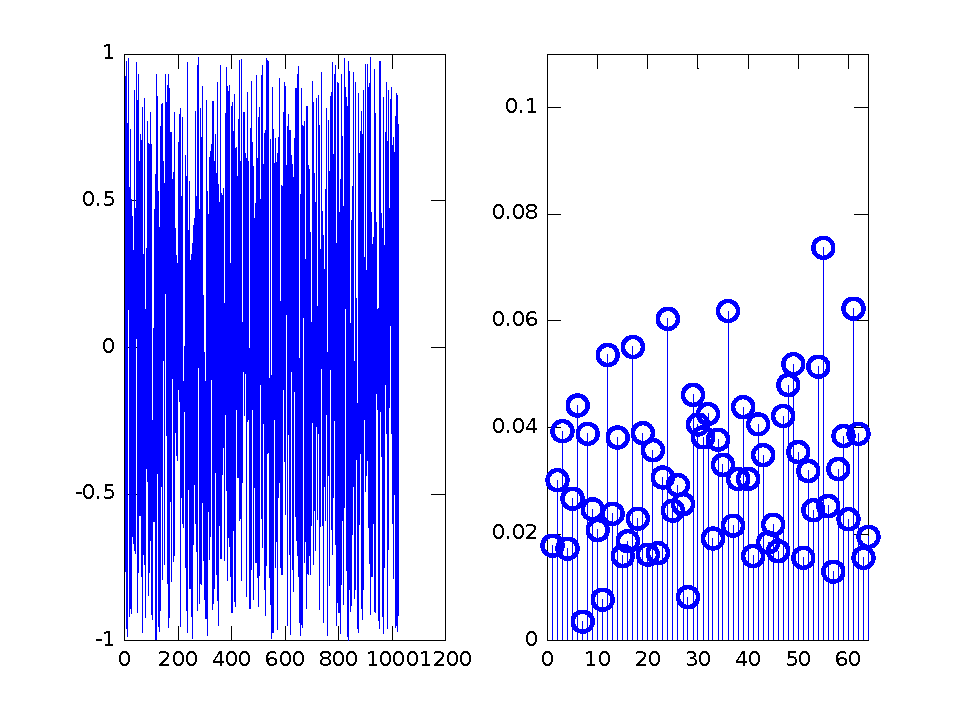
\includegraphics[width=0.8\textwidth]{\plotdir/conv_noise_and_saw_1}
   \end{center}
	\caption{Rumore bianco nel dominio del tempo e in quello della frequenza\label{fig:white noise}}
\end{figure}

Usiamo un'onda a dente di sega (rappresentata in Fig.\vref{fig:sawtooth}) come
risposta all'impulso.

\begin{figure}[hbt]
  \begin{center}
	  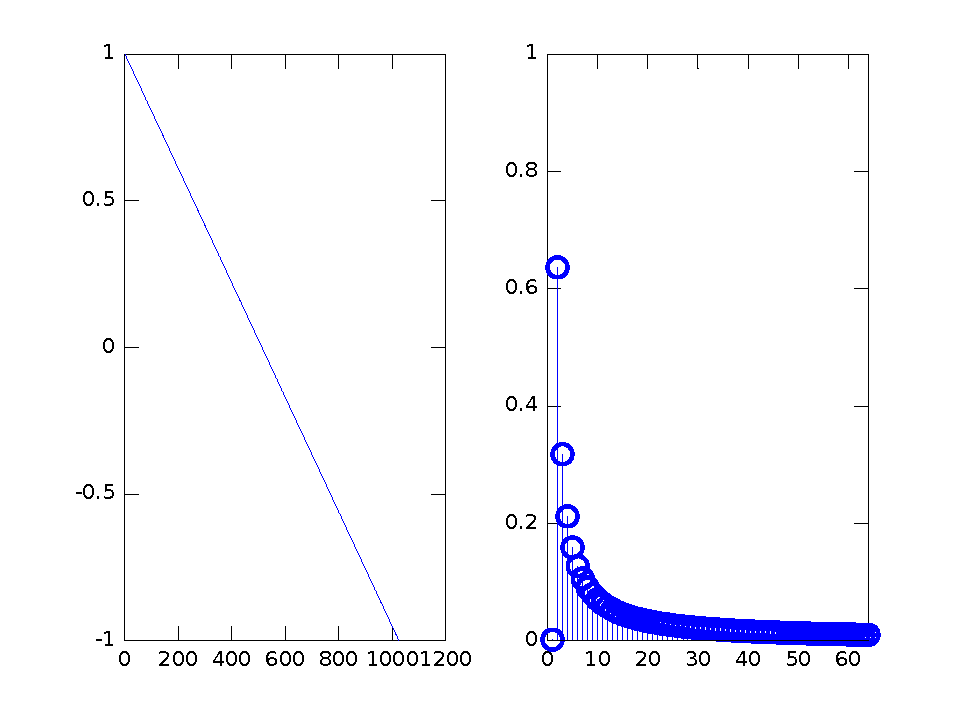
\includegraphics[width=0.8\textwidth]{\plotdir/conv_noise_and_saw_2}
  \end{center}
	\caption{Onda a dente di sega nel dominio del tempo e in quello della frequenza\label{fig:sawtooth}}
\end{figure}

Convolvendo il rumore bianco per l'onda a dente di sega otterremo la
moltiplicazione delle magnitudini delle due rappresentazioni spettali (cf.
Fig.\vref{fig:noise and saw convolved}),

\begin{figure}[hbt]
  \begin{center}
	  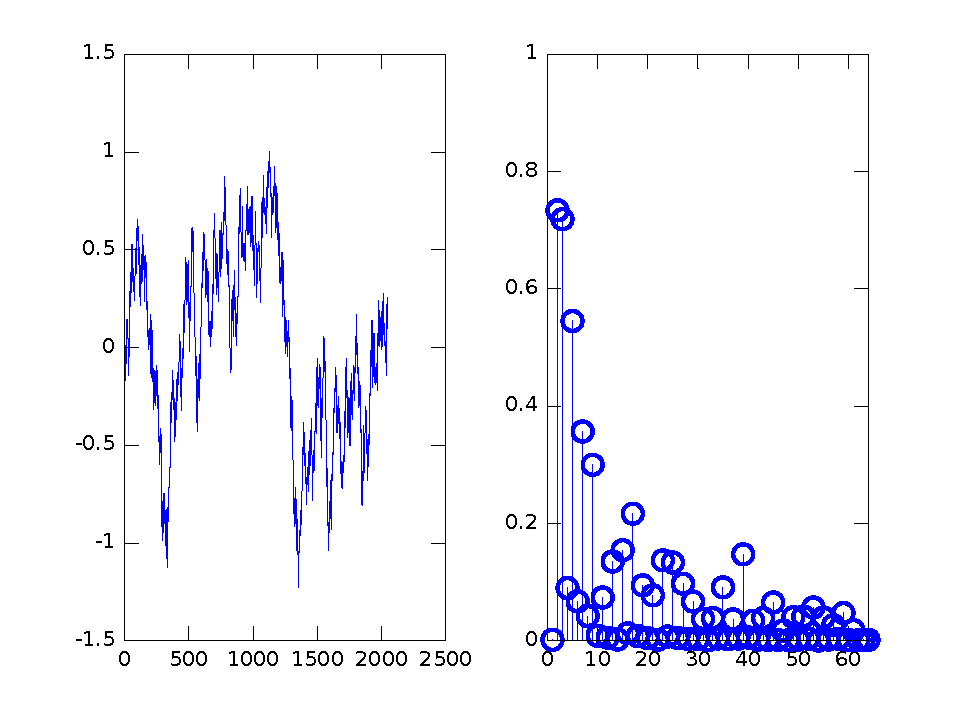
\includegraphics[width=0.8\textwidth]{\plotdir/conv_noise_and_saw_3}
  \end{center}
	\caption{Convoluzione dei due segnali\label{fig:noise and saw convolved}}
\end{figure}

Il codice {\tt matlab/octave} che produce questi grafici \`e riportato qui di
seguito:

\verbatiminput{\plotdir/conv_noise_and_saw.m}
